% $Header: /cvsroot/latex-beamer/latex-beamer/solutions/conference-talks/conference-ornate-20min.en.tex,v 1.7 2007/01/28 20:48:23 tantau Exp $

\documentclass[10pt]{beamer}



\mode<presentation>
{
  \usetheme{Berkeley}
  % or ...

  \setbeamercovered{transparent}
  % or whatever (possibly just delete it)
}


\usepackage[english]{babel}
% or whatever

\usepackage[latin1]{inputenc}
% or whatever

\usepackage{times}
\usepackage{graphicx}

\usepackage{tikz}
\usepackage{lineno}
\usepackage[english]{babel}
\usepackage{seqsplit}
\usepackage[nottoc]{tocbibind} 
\usepackage[utf8]{inputenc}
\usepackage{amsmath}
\usepackage{amssymb}
\usepackage{amsthm}
\theoremstyle{plain} % insert bellow all blocks you want in italic


\title[Part C Dissertation] % (optional, use only with long paper titles)
{Extensions of number fields with small ramification}

\subtitle
{}

\author % (optional, use only with lots of authors)
{Samuel Bodansky}


\institute % (optional, but mostly needed)
{
  University of Oxford
  }
.

\date % (optional, should be abbreviation of conference name)
{February 2019}
\setbeamertemplate{sidebar right}{}
\setbeamertemplate{footline}{%
\hfill\usebeamertemplate***{navigation symbols}
\hspace{1cm}\insertframenumber{}/\inserttotalframenumber}

\begin{document}

\begin{frame}
  \titlepage
\end{frame}
\begin{frame}{Contents}
\tableofcontents
\end{frame}

\section{Goal}
\begin{frame}{Aim of Project}
Goal: For a given number field K, what is the maximal unramified extension $K^{ur}$ of K is and also to calculate $\Gamma(K^{ur}:K)$

\end{frame}

\section{Class Field Theory}

\begin{frame}{Motivation}
\begin{definition}
A prime ideal $\mathfrak{p}$ in $\mathcal{O}_K$ factors in an extension L of K as
$\mathfrak{p}\mathcal{O}_L=\mathfrak{B}_1^{e_1}...\mathfrak{B}_m^{e_m}$, where $\mathfrak{B}_i$ are ideals in $\mathcal{O}_L$ intersecting $\mathcal{O}_K$ at $\mathfrak{p}$. Note ach $e_i\geq1$ and if $e_i>1$ for some i then we say that $\mathfrak{p}$ ramifies in L. If $e_i=1$ for all i then we say $\mathfrak{p}$ splits in L.
\end{definition}
    \begin{theorem}
The compositum of two finite unramified extensions of K is also unramified, and so the union $K^{ur}$ of all unramified extensions is also an unramified extension of K.
\end{theorem}
\begin{definition}
h(K) is the \textbf{Hilbert class field} of K. It is maximal abelian extension, L of K unramified at all primes of K. The degree of its extension over K is equal to the class number of K, and its Galois group is isomorphic to the ideal class group of K.
\end{definition}
\end{frame}
\begin{frame}{Hilbert Class Fields}
  \begin{definition}
The \textbf{Hilbert Class Tower} is $K_H=\bigcup_{i}K_{i}$. It is often very useful to consider when this tower ends. If K is a UFD, then K is equal to its own Hilbert class field.  
\end{definition}
    \begin{example}
    Suppose K=$\mathbb{Q}$. Then K is its own Hilbert class field. 
\end{example}
\begin{example}
    Suppose $K=\mathbb{Q}[\sqrt{-5}]$, and take $L=\mathbb{Q}[\sqrt{-1},\sqrt{-5}]$. L is an unramified degree 2 extension of K and so the Hilbert class field of K is $K[\sqrt{-1}]$.
\end{example}

\end{frame}
\section{$\mathbb{Q}$,P-adics and Cyclotomics}
\subsection{Examples in $\mathbb{Q}$}
\begin{frame}{Extensions of $\mathbb{Q}$}
    \begin{theorem}
     Suppose that K be a field extension of $\mathbb{Q}$ with discriminant D. Then a prime p
ramifies in K if and only if $p|D$.   
    \end{theorem}
    \begin{corollary}
A field extension K of $\mathbb{Q}$ ramifies at precisely one prime iff the absolute value of disc(K) is a prime power.
\end{corollary}
\begin{example}
    Suppose $f(x)=x^5-5x^4-2x^3+x^2-3x+1$, and K is the splitting field of f over $\mathbb{Q}$. Then $disc(K)=-3442951=151^3$ and so 151 is the only prime which ramifies in K over $\mathbb{Q}$. Note that f(x) is an irreducible quintic with precisely three real roots, meaning that $\Gamma(K/\mathbb{Q})\cong\ S_5$ and K is an unsolvable extension of $\mathbb{Q}$.
\end{example}
\end{frame}
\subsection{P-adics and Cyclotomics}
\begin{frame}{P-adics results}

\begin{theorem}
   Suppose $\zeta$ is an $n^{th}$ root of unity. Let K be a number field, $L=K(\zeta)$. 
L is a degree n unramified extension of K. 
\end{theorem}

Let $\zeta$ be a primitive n-th root of unity, with $n=kp^{m}$, (k,p)=1.
\begin{example}[Field Inclusions]
      $\mathbb{Q}_{p}=K\subseteq K^{tur}=K(\zeta_k)\subseteq K^{ur} = K^{tur}(\zeta_{p})\subseteq K(\zeta_n)$
\end{example}
\begin{lemma}
Suppose p is a prime and gcd(n,p)=1. Then there exists $m\in\mathbb{N}$ such that $n|p^m-1$.
\end{lemma}
\begin{theorem}
    Let $K=\mathbb{Q}_p$. Then $K^{ur}$ is K adjoined with all roots of unity with order prime to p. 
\end{theorem}

\end{frame}
\begin{frame}{Odlyzko's Bounds}
\begin{definition}
$rd_K$ is the root discriminant of K, $|d_K|^\frac{1}{n_K}$
\end{definition}
\begin{lemma}
 If L is an unramified extension of K, then L and K have the same root discriminant.
\end{lemma}
    Odlyzko's Bound improved on the bounds for Minkowski for the discriminant of a number field. Moreno states it as  
\begin{equation}
rd_K\geqslant 60^{\frac{r_1}{n}}22^{\frac{r_2}{n}}e^\frac{-8.6}{n^(2/3)}\end{equation}
Furthermore, under the assumption of the Generalised Riemann Hypothesis, 
this bound can be improved by replacing the numbers 60 and 22 by 188 and 41 respectively. 
\end{frame}
\begin{frame}{Quadratic Number Fields}
    Let $K=\mathbb{Q}(\sqrt{d})$. Using Odlyzko's bound and the above lemma, for $|d|<499(2003)$, we have $[K^{ur}:K]$ is finite. If $[K^{ur}:K_H]<60$, then $K^{ur}=K_H$.\par
    Yamamura  calculates $\Gamma(K^{ur}:K)$ for $|d|<719$ when $K^{ur}\neq K_1$.\par
    Sometimes to calculate higher up the tower we can use the tower law where $K_g$ is the genus field of K: \begin{equation}
    [K_2:\mathbb{Q}] = [K_2:(K_g)_1]h(K_g)[(K_g)_1:\mathbb{Q}]
\end{equation}\par
\begin{example}
For d=-255, $K_H=K_2$. We have $cl(K)\equiv C_6\times C_2$, $K_1 = K\lb\sqrt{5},\sqrt[3]{(9+\sqrt{85})/2}\rb$, and $K_2 = K_1\lb\sqrt{2+\sqrt{5}\lb5+2\sqrt{-3}}\rb\rb$. Here $\murgg \cong Q_8 \times C_3$.
\end{example}

\end{frame}
\begin{frame}{Cubic Extensions (Wong) }
 $K=\mathbb{Q}(\theta)$ where $\theta$ is a root of a cubic
f(x). If $\Gamma(K/\mathbb{Q}) \cong C_3$, call K a  \textbf{cyclic cubic field}.
\begin{theorem}[Galois Theory]
Then K is a cyclic cubic field iff disc(f) is a square. 
\end{theorem}
\begin{example}
    Let $f=x^3-x^2-2x+1$. Then disc(K)=$7^2$, $rd_{k}=3.66$ and h(K)=1. Unconditionally, K does not have an unsolvable unramified extension, $\Gamma(K:\mathbb{Q})\cong C_3$
\end{example}
\end{frame}
\begin{frame}{Cubic Calculation Example}
    Wong now gives examples of how to calculate the maximal unramified extension of a cyclic cubic field with nontrivial class number. \begin{example}
    $f=x^3-x^2-54x+169$, disc(K)=$163^2$, $rd_{k}=29.84$. Here we have h(K)=4.\par Define $g(x)=x^6-3x^5-11x^4+27x^3-3x^2-11x+1$. Then John Jones' website gives $L = split(g,\mathbb{Q})$ with $\Delta(K_1)=163^4$.\par Firstly $\Gamma(L/\mathbb{Q}) \cong A_4$, and 163 is unramified in $L/K$. Hence indeed $L=K_1$.\par  We know that $\Gamma(L/K)\cong V_4$ which is a normal subgroup of $A_4$. \par Now h(L)=1 and $rd_K < 54.62$ which is the lower bound for the root discriminant of totally real fields of degree 720, so $\Gamma(K^{ur}/K) \cong V_4$ and $\Gamma(K^{ur}/\mathbb{Q}) \cong A_4$. 
\end{example}
\end{frame}

\begin{frame}{Serre: Quartic Number Field}
Define  \begin{equation}
    f(x)=x^4-x-1, \Delta(f)=-283
\end{equation}
Note f has two real and two imaginary roots. Let  L be the splitting field of f and $\Gamma(L/\mathbb{Q})\cong S_4$.\par
By the FTGT, there exists an intermediate field H corresponding to the normal subgroup $V_4$ of $S_4$. \par 
Now $L^H$ is the Hilbert class field of $K= \mathbb{Q}(\sqrt{-283})$ and h(K)=3. Now define a further field extension of L, M such that M is unramified over L (and hence also over K) and M is a Galois extension of $\mathbb{Q}$.  
\par Martinet proved that M is the maximal unramified extension of K, $\Gamma(M/K)\cong SL_2(F_3)$ of order 24. In addition, $\Gamma(M/\mathbb{Q})\cong GL_2(F_3)$. 
\end{frame}

\begin{frame}{Primes of the form $x^2+ny^2$}
    \begin{corollary}
Suppose $K=\mathbb{Q}{\sqrt{-n}}$ n is positive,squarefree, $n\not\equiv 3(4)$, so that $d_K=-4n$. If p is an odd prime not dividing n, then
\begin{equation} p=x^2+ny^2 \Longleftrightarrow p\:splits\:completely\:in\:the\:Hilbert\:class\:field\:of\:K.
\end{equation}
Hence the primes of the form $x^2+ny^2$ characterise the Hilbert class field of $\mathbb{Q}(\sqrt{-n})$.
\end{corollary}
\end{frame}

\section{Infinite Unramified Extensions}

\begin{frame}{The Hilbert p-class Field and Finite Extensions}
    \begin{Theorem}
If any p-class field tower over K is infinite, then the class field tower is also infinite. If the p-class tower terminates, then $H_{K_\infty}^{p}$ is a finite field extension of K and $\Gamma(H_{K_\infty}^{p}/K)$ is a p-group.
\end{Theorem}
Converse not necessarily true; $\mathbb{Q}(\sqrt{-239},\sqrt{4049})$. Then this biquadratic field extension of $\mathbb{Q}$ has an infinite class field tower, but all p-class field towers are finite. 
\end{frame}

\begin{frame}{Infinite p-class Tower Examples}
\begin{example}
    Define $K=\mathbb{Q}(\sqrt{-3.5.7.11.19.23})$. Then 6 odd primes ramify in K over $\mathbb{Q}$, and so K has an infinite 2-class field tower. 
\end{example}
\begin{example}[Schoof]
$\mathbb{Q}(\sqrt{-191.773})$ has an infinite 2-class field tower. There are infinitely many real quadratic number fields of the form $\mathbb{Q}(\sqrt{p_1.p_2})$ with $p_1$ and $p_2$ prime, possessing infinite class field towers. 
\end{example}
\end{frame}
\section{Infinite unramified extensions}
\begin{frame}{Example of Unsolvable Unramified Extension}
K is a class field, h(K)=1. Then K has no abelian.
K may have a non-solvable unramified extension.
\begin{equation}
   K=\mathbb{Q}(\sqrt{29},\sqrt{4967}) 
\end{equation}
\begin{equation}
   L=split(x^7 - 11x^5 + 17x^3 - 5x + 1,\mathbb{Q}[x])
\end{equation}
Then K has class number 1 and L is a PSL(2, 7)-extension of K.
Maire showed that there exist biquadratic number fields with class number one with an infinite unramified extension.
\end{frame}

\begin{frame}{Field Extension Diagram-Brink}
  \begin{center}
    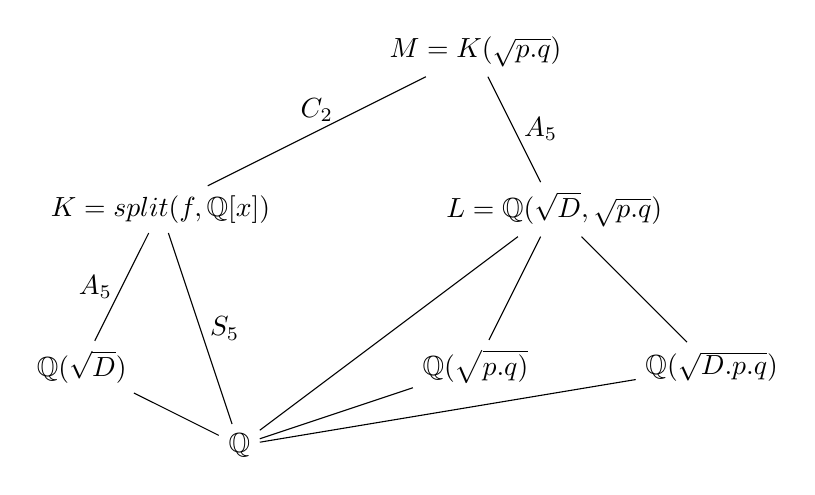
\begin{tikzpicture} [align=center]
  \path  (0, 0)   node(Q)  {$\mathbb{Q}$}
          +(6, 1)   node(QD12) {$\mathbb{Q}(\sqrt{D.p.q})$}
          ++(3,1)   node(Q12) {$\mathbb{Q}(\sqrt{p.q)}$}
           ++(-5,0)   node(QD) {$\mathbb{Q}(\sqrt{D})$}
           ++(1,2)   node(K) {$K=split(f,\mathbb{Q}[x])$}
           ++(5,0)   node(L) {$L=\mathbb{Q}(\sqrt{D},\sqrt{p.q})$}
            ++(-1,2)   node(M) {$M=K(\sqrt{p.q})$};
    \draw [-] (Q) to node [pos=0.5,above]{} (Q12);
    \draw [-] (Q) to node [pos=0.8,below]{} (QD);
    \draw [-] (Q) to node [pos=0.5,below]{} (QD12);
  \draw [-] (QD) to node [pos=0.5,left]{$A_5$} (K);
  \draw [-] (Q) to node [pos=0.5,right]{$S_5$} (K);
  \draw [-] (Q) to node [pos=0.5,below]{} (L);
  \draw [-] (Q12) to node [pos=0.5,below]{} (L);
  \draw [-] (QD12) to node [pos=0.5,below]{} (L);
    \draw [-] (L) to node [pos=0.5,right]{$A_5$} (M);
     \draw [-] (K) to node [pos=0.5,above]{$C_2$} (M);
\end{tikzpicture}
\end{center}  
\end{frame}
\section{Bounds on Discriminants}


\begin{frame}{Examples of Suitable Polynomials and Primes}
Using Odlyzko's bounds and computer search, we find 
\begin{example}
$f(x)=x^5+4x^4-6x^2-x+1, p=1531,q=71,151,227,\Delta(f)=170701$
\end{example}
    \begin{example}
$ f(x)=x^5-4x^4+12x^2-8x+1,p=1987,q=31,107,211,239,\Delta(f)=186037$
\end{example}
The class number of the splitting fields of each of these polynomials is 1; they are equal to their own Hilbert class fields.  
\end{frame}
\section{Yamamoto's Results}
\begin{frame}{Polynomials of the form $x^n+ax+b$}
       $ f(x) = x^n+ax+b \in \mathbb{Z}[x]$,
$K=split(f,\mathbb{Q})$
If :
\begin{enumerate}
    \item $(n-1).a$ and $n.b$ are relatively prime 
    \item $\Gamma(K/\mathbb{Q}) \cong S_n$
\end{enumerate}\par
Then K is an $A_n$-extension of $\mathbb{Q}(\sqrt{\Delta(f)})$ which is unramified at all finite primes. \begin{example}
$f(x) = x^5-x+1$, then $\Delta(f)= 2869$, $L = \mathhbb{Q}(\sqrt{2869})$. Then K is unramified over L and $\Gamma(K:L)\cong A_5.$
\end{example}  
\end{frame}
\begin{frame}{Serre: Cubic Number Field}
 \begin{equation}
 f(x)=x^3-x-1, \Delta(f)=-23
\end{equation}
 f has one real root and two imaginary roots. Let L denote its splitting field. Then $\Gamma(L/\mathbb{Q})\cong S_3$ and it is a degree three extension of the quadratic field $K= \mathbb{Q}(\sqrt{-23})$.  h(K)=3 and Odlyzko's bounds show that $L=K^{ur}$.
  \begin{center}
    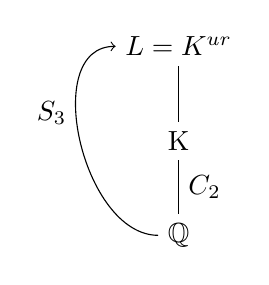
\begin{tikzpicture}[node distance = 1.2cm, auto]
      \node (Q) {$\mathbb{Q}$};
      \node (K) [above of=Q] {K};
      \node (L) [above of=K] {$L=K^{ur}$};
    \draw [->,out=180,in=180,looseness=1] (Q.west) to node[above][pos=0.6,left]{$S_3$}  (L.west);    
    \draw [-] (Q) to node [pos=0.5,right]{$C_2$} (K);
        \draw [-] (K) to node [pos=0.1,left]{} (L);
      \end{tikzpicture}
\end{center}
\end{frame}

\begin{frame}{Kondo}
    \begin{theorem}
   F is a degree n number field with squarefree discriminant.  d(F) of degree n, Galois closure K. Then \begin{enumerate}
        \item $\Gamma(K:\mathbb{Q})\cong S_n$
        \item $K/\mathbb{Q}(\sqrt{d(F)})$ is an unramified extension.
    \end{enumerate}
\end{theorem}
\end{frame}
\begin{frame}{Example}
\begin{example}
 $f(x)=x^6 + x^5 - 6x^4 - 4x^3 + 8x^2 + 3x - 2$. Also define $F=\mathbb{Q}(\theta)$, where $\theta$ is a root of f, $K=split(f,\mathbb{Q})$. Then we get $d(f)=\Delta(F)=7846061=17^3.1597$. 
\begin{equation}
   f(x)= (x^3 + 9x^2 + 16x + 7)^2\:modulo\:17
\end{equation}
By the above, we see that K is an unramified extension of $\mathbb{Q}(\sqrt{17^3.1597})$. Also, $\Gamma(K/\mathbb{Q})\cong S_3 \wr C_2$. Furthermore $K/\mathbb{Q}(\sqrt{17^3.1597})$ is unramified with Galois group isomorphic to the Frobenius group of order 36.
\end{example}    
\end{frame}
\begin{frame}{Summary}
    \begin{enumerate}
        \item The theory of maximal unramified extensions is fairly well understood for p-adics and cyclotomics
        \item There are applications of Hilbert Class Field theory to primes of the form $p^2=x^2+ny^2$ but and this is very well understood. 
         \item Odlyzko's bounds can show strong results about imaginary quadratic number fields, and some biquadratic number fields. They can also be applied for some number fields defined by polynomials. 
         \item Serre gives some examples for calculating $K^{ur}$ in some specific situations but there is no general formula. 
         
    \end{enumerate}
\end{frame}
\end{document}
